\section{Benefits of Small Tasks}
\subsection{Running real-time and batch jobs together}
\kay{how can we quantify this?}
\subsection{How do small tasks affect stragglers?}
Breaking jobs into many waves of tiny tasks can improve completion time by 5x or more.  We assume task runtimes are exponentially distributed: some tasks take much longer than others due to resource contention on the machine, resource contention over the network, data skew, etc.  If tasks are all run in a single wave, the runtime of the job will be much longer than the mean task runtime, because the job is limited by the \emph{last} task to complete.  To measure the impact of breaking tasks up into a large number of tiny tasks, we assume jobs have a constant number of ''slots'' available, where a slot may represent a machine, or a fair share of the cluster allocated to the user who initiated the job.  we assume that if we break a task with mean runtime $x$ into k tiny tasks, each tiny task will have mean runtime $x/k$.  Figure~\ref{fig:outliers} demonstrates the impact of breaking a job with a single wave of tasks into $k$ times as many tiny tasks, for different values of $k$ (shown along the x-axis).  Response times are normalized relative to the response time for the job when run in a single wave.  We measure this impact for varying number of slots available to the job.  As expected, jobs with 1 slot see no improvement, but as the number of slots increases, jobs see as much as a 5x (eyeballed) improvement in response time from breaking tasks into tiny sub-tasks. This improvement justifies using a large number of tasks even if the overhead of starting a task is high; as long as the overhead of starting a task is less than 4x the task's completion time (we expect $<10$\% overhead), using tiny tasks will improve over running tasks in a single wave.

\begin{figure}[t]
\centering
\hspace{2ex}
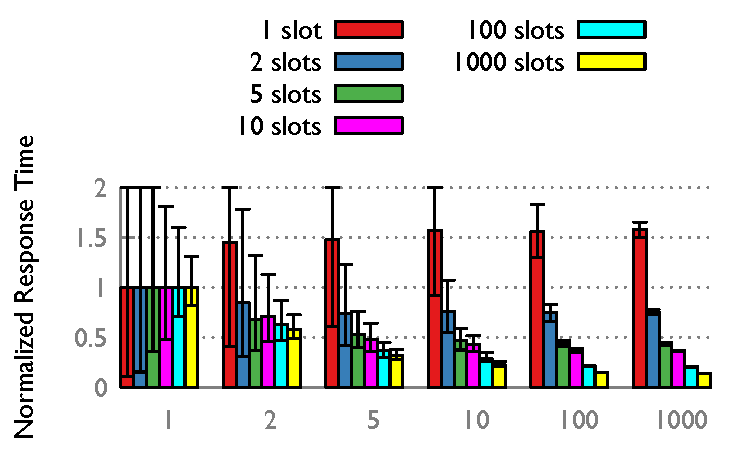
\includegraphics[width=0.5\textwidth]{figures/results_stragglers}
\vspace{-4ex}
\caption{Improvement in job completion time from breaking tasks into a large number of ``tiny tasks.'' \kay{need to fix 1-slot bars, which are screwed up, as well as nauseating colors}}
\vspace{-2ex}
\label{fig:outliers}
\end{figure}

TODO: use different original distributions of task duration

\subsection{How much do smaller tasks improve load balancing?}
two improvements on the load balancing front:
\begin{itemize}
\item File accesses: with smaller tasks, each task accesses a much smaller portion of a file.  In the context of Hadoop MapReduce, this would mean using much smaller HDFS file blocks.  With smaller blocks, the law of large numbers dictates that file accesses will be spread more evenly over machines than with large blocks.  To understand this affect, we use traces from Facebook's datacenter to obtain a distribution of the number of accesses per file.  We then randomly assign file blocks to machines, and measure the number of block accesses per machine, over 30 second intervals.\kay{should use smaller intervals? this would exacerbate affect, and you really care about how many accesses happen concurrently with yours, so 1s intervals could be realistic}  We divide files into smaller and smaller blocks (multiplier = 1 indicates block sizes equal to Facebook's current block size; multiplier = 10 indicates that we have block sizes 1/10th the size of Facebook's), to understand how smaller blocks improve load balancing.  With perfect load balancing, we would expect all machines to have the exact same number of file accesses.  Figure~\ref{fig:data_skew} demonstrates that even using 10 times as many tasks decreases 95th percentile machine load by 25\%\footnote{totally eyeballed from figure}.  \kay{we should simulate larger multipliers; my machine just died at 10}

\begin{figure}[t]
\centering
\hspace{2ex}
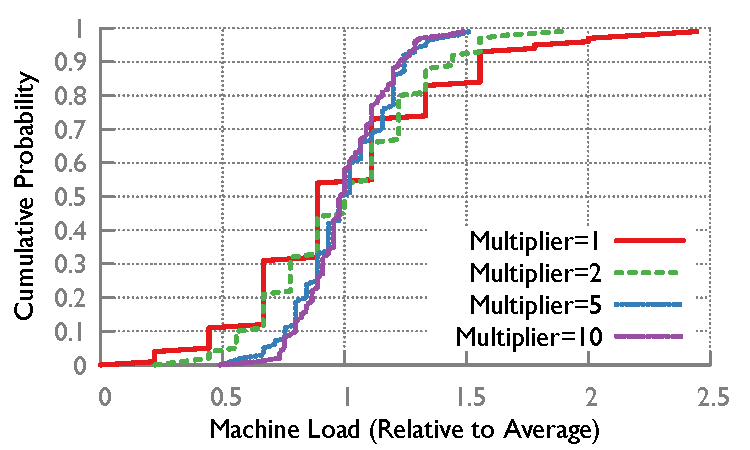
\includegraphics[width=0.5\textwidth]{figures/skew_results}
\vspace{-4ex}
\caption{Effect of decreasing file block size on the distribution of file accesses across machines.}
\vspace{-2ex}
\label{fig:data_skew}
\end{figure}

\item Network congestion: first, no huge flows (since all tasks are limited in how much data they use). This leads to essentially the same phenomenon as above.
\end{itemize}

\subsection{How do small tasks affect data skew?}
Many small tasks, so don't have to worry that one reducer (or other intermediate phase) has a ton of data.  Still need to worry about splitting very popular keys though...

\subsection{How does balance of tasks in a cluster (measured by queue length ?) change as we change granularity?}
\kay{Shivaram, what did you mean by this?}